\documentclass[8pt,fleqn]{beamer}

%---------------------------------------------------------------
% Macros
% version 3 by Igor Ruiz-Agundez 2011
% version 2 by Jakob Suckale 2007
% version 1 by Harish Bhanderi 2002
%---------------------------------------------------------------

% This file contains macros that can be called up from connected TeX files
% It helps to summarise repeated code, e.g. figure insertion (see below).


%---------------------------------------------------------------
% MY COMMANDS
%---------------------------------------------------------------
%MY COMMANDS
\newcommand{\sub}[1]{\mbox{\scriptsize{#1}}}
\newcommand{\der}[2]{ \frac{ \partial #1 }{\partial #2} }
\newcommand{\dtot}[2]{ \frac{ d #1 }{d #2} }
\newcommand{\pr}[1]{ \left( #1 \right) }
\newcommand{\cor}[1]{ \left[ #1 \right] }
\newcommand{\lla}[1]{ \left\{ #1 \right\} }
\newcommand{\eq}[2]{\begin{equation} \label{#1} #2 \end{equation}}
\newcommand{\bds}[1]{\boldsymbol{ #1 }}
\newcommand{\oiint}{\displaystyle\bigcirc\!\!\!\!\!\!\!\!\int\!\!\!\!\!\int}
\newcommand{\mathsize}[2]{\mbox{\fontsize{#1}{#1}\selectfont $#2$}}
\newcommand{\sinc}[1]{\mbox{sinc}#1}

\newcommand{\cita}[1]{\textsuperscript{\tiny\cite{#1}}}
\newcommand{\ket}{\rangle}
\newcommand{\bra}{\langle}

\renewcommand{\listtablename}{Índice de tablas}
\renewcommand{\tablename}{Tabla}

\usepackage{color, colortbl}
%Celda de colores en tablas
\newcommand{\cellc}[1]{\multicolumn{1}{|>{\columncolor[rgb]{0.8, 0.8, 0.8}}c|}{#1}}

%---------------------------------------------------------------
% Figures
%---------------------------------------------------------------


% Makes the \InsertFig macro compatible both with one or two columns
\makeatletter
\newlength \figwidth
\if@twocolumn
  \setlength \figwidth {\columnwidth}
\else
  \setlength \figwidth {\textwidth}
\fi
\makeatother

% \InsertFig allows inserting figures
% Parameters
% 1 --> Filename
% 2 --> Label for referencing
% 3 --> Title describing the figure (caption)
% 4 --> Description of the figure
% 5 --> Figure width, range [0,1]. If parameter is left blank the figure size is not change
% 6 --> Any other option for \includegraphics
% Usage:
% \InsertFig{}{}{}{}{}{}
%
\newcommand{\InsertFig}[6]{%
	\ifthenelse{\isempty{#5}}%
	{% if #1 is empty
		\begin{figure}[htbp!]
		\centering
		\includegraphics[#6]{#1}%
		\caption{#3}{\textbf{#4}}
		\label{#2}
		\end{figure}    
	}
	{% if #1 is not empty
		\begin{figure}[htbp!]
		\centering
		\includegraphics[width=#5\figwidth,#6]{#1}%
		\caption{#3}{\textbf{#4}}
		\label{#2}
		\end{figure}
	}
}

%% Simple version of \InsertFig
%\newcommand{\InsertFig}[5]{
%  \begin{figure}[htbp]
%   	\centering
%    \includegraphics[width=#4\textwidth,#5]{#1}%
%    \caption{#3}
%    \label{#2}
%  \end{figure}
%}



% insert a centered figure with caption
% parameters 1:filename, 2:label, 3:title, 
\newcommand{\figuremacro}[3]{
	\begin{figure}[htbp]
		\centering
		\includegraphics[width=1\textwidth]{#1}
		\caption[#3]{\textbf{#3}}
		\label{#2}
	\end{figure}
}


% insert a centered figure with caption and description
% parameters 1:filename, 2:label, 3:title, 4:description
\newcommand{\figuremacroD}[4]{
	\begin{figure}[htbp]
		\centering
		\includegraphics[width=1\textwidth]{#1}
		\caption[#3]{\textbf{#3} - #4}
		\label{#2}
	\end{figure}
}

% insert a centered figure with caption and description AND WIDTH
% parameters 1:filename, 2:label, 3:title, 4:description, 5: textwidth
% textwidth 1 means as text, 0.5 means half the width of the text
\newcommand{\figuremacroDW}[5]{
	\begin{figure}[htbp]
		\centering
		\includegraphics[width=#5\textwidth]{#1}
		\caption[#3]{\textbf{#3} - #4}
		\label{#2}
	\end{figure}
}

% inserts a figure with wrapped around text; only suitable for NARROW figs
% o is for outside on a double paged document; others: l, r, i(inside)
% text and figure will each be half of the document width
% note: long captions often crash with adjacent content; take care
% in general: above 2 macro produce more reliable layout
\newcommand{\figuremacroN}[3]{
	\begin{wrapfigure}{o}{0.5\textwidth}
		\centering
		\includegraphics[width=0.48\textwidth]{#1}
		\caption[#2]{{\small\textbf{#2} - #3}}
		\label{#1}
	\end{wrapfigure}
}




% Estas definiciones son para el comando \InsertFigBox
\newlength{\anchoFigura}
\newlength{\anchoFloat}
\addtolength{\fboxsep}{2\fboxsep}
%\renewcommand{\capfont}{\normalfont\normalcolor\sffamily\small}
%\renewcommand{\caplabelfont}{\normalfont\normalcolor\sffamily\bfseries\small}

% El comando \InsertFigBox nos permite insertar figuras en un marco
% Los parametros son:
% 1 --> Fichero de la imagen
% 2 --> Etiqueta (label) para referencias
% 3 --> Texto a pie de imagen
% 4 -> Porcentaje del ancho de página que ocupará la figura (de 0 a 1)
% 5 --> Opciones que queramos pasarle al \includegraphics
\newcommand{\InsertFigBox}[5]{%
  \setlength{\anchoFloat}{#4\textwidth}%
  \addtolength{\anchoFloat}{-4\fboxsep}%
  \setlength{\anchoFigura}{\anchoFloat}%
  \begin{figure}%
    \begin{center}%
      \Ovalbox{%
        \begin{minipage}{\anchoFloat}%
          \begin{center}%
            \includegraphics[width=\anchoFigura,#5]{#1}%
            \caption{#3}%
            \label{#2}%
          \end{center}%
        \end{minipage}
      }%
    \end{center}%
  \end{figure}%
}



%---------------------------------------------------------------
% Misc
%---------------------------------------------------------------

% predefined commands by Harish
\newcommand{\PdfPsText}[2]{
  \ifpdf
     #1
  \else
     #2
  \fi
}


%---------------------------------------------------------------
% Locales
%---------------------------------------------------------------


%%
%% Para quitar traducciones raras (Cuadros)
%% A de usarse cada vez que se seleccione el idioma
%%
\newcommand{\MejorarTraducciones}{%
       \renewcommand{\listtablename}{Índice de tablas}
       \renewcommand{\tablename}{Tabla}
       \renewcommand{\lstlistingname}{Lista}
}%



%---------------------------------------------------------------
% Source code
%---------------------------------------------------------------


%%
%% Para escribir extractos de codigo
%%
%% Las tabulaciones se substituyen por dos espacios
%\fvset{tabsize=2}
%% Creamos un nuevo environment de fancyvrb para los ejemplos enmarcados
%\DefineVerbatimEnvironment{VerbEj}{BVerbatim}{fontsize=\small,samepage=true,commandchars=\\\{\}}
%% Colo de fondo
%\definecolor{grisfondo}{gray}{0.9}
%% Environment para extractos de codigo
%\newenvironment{codigo}%
%{\VerbatimEnvironment\begin{Sbox}\begin{VerbEj}}%
%{\end{VerbEj}\end{Sbox}\setlength{\fboxsep}{8pt}\begin{center}\fcolorbox{black}{grisfondo}{\TheSbox}\end{center}}
%
%% Otro formato más bonito para código fuente
%\newcommand{\codigofuente}[3]{%
%  \lstinputlisting[language=#1,caption={#2}]{#3}%
%}






\title{\textbf{The place of the Milky Way and Andromeda in the cosmic web} \\ .\\ 
\small{Sebastian Bustamante Jaramillo\\ 
Grupo de Física y Astrofísica Computacional, FACom\\
Instituto de Física - Universidad de Antioquia \\ .\\  
\textbf{Asesor:} Jaime Forero -- Universidad de los Andes \\
\textbf{Co-asesor:} Jorge Zuluaga -- Universidad de Antioquia}
\author[Sebastian Bustamante]{}}
\institute[FACom]{}


\begin{document}
\justifying


%=================================================================================================================
\begin{frame}
\titlepage
\end{frame}
%=================================================================================================================
\begin{frame}
\begin{block}{Tabla de Contenidos}
\

	\tableofcontents	

\	
\end{block}
\end{frame}

%*****************************************************************************************************************
%			MOTIVACION
%*****************************************************************************************************************
\section{Motivación}
\label{sec:motivo}
%=========================================================================
%FRAME 3
\begin{frame}
\begin{block}{Motivación}\justifying
%.........................................................................
%Vweb
\begin{figure}[htbp]
	\centering
	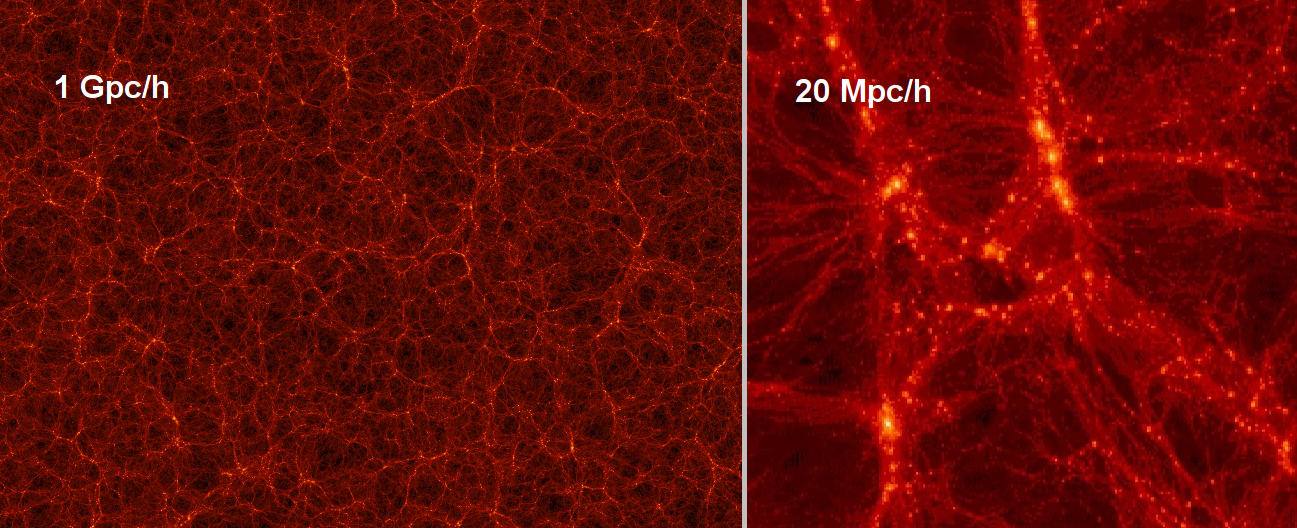
\includegraphics[trim = 0mm 0mm 0mm 0mm, clip, width=1.0\textwidth]
	{./figures/Web.png}
\end{figure}
%.........................................................................
\end{block}
\end{frame}
%=========================================================================
%FRAME 4
\begin{frame}
\begin{block}{Motivación}\justifying

\begin{itemize}
\item Cuantificar la estructura de la red cósmica y reproducir su apariencia 
visual.
\item En trabajos recientes se han realizado estudios de la influencia del 
entorno en propiedades físicas de halos de materia oscura.
\item Extender este tipo de estudios a sistemas como el grupo local.
\item Identificar sistemas tipo grupo local en simulaciones cosmológicas de 
materia oscura.
\item El grupo local de galaxias es el sistema a escala cosmológica mejor 
conocido.
\item Algunos tests del modelo de concordancia $\Lambda CDM$ son realizados 
en el grupo local.
\end{itemize}

\end{block}
\end{frame}
%=========================================================================
%FRAME 5
\begin{frame}
\begin{block}{Motivación}\justifying
%.........................................................................
%Local Group
\begin{figure}[htbp]
	\centering
	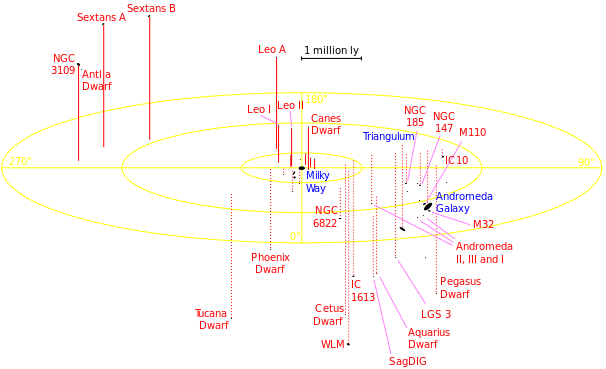
\includegraphics[trim = 0mm 0mm 0mm 0mm, clip, width=0.8\textwidth]
	{./figures/LocalGroup.png}
\end{figure}
%.........................................................................
\end{block}
\end{frame}
%=========================================================================
%FRAME 6
\begin{frame}
\begin{block}{Motivación}\justifying
%.........................................................................
%Pairs in Web
\begin{figure}[htbp]
	\centering
	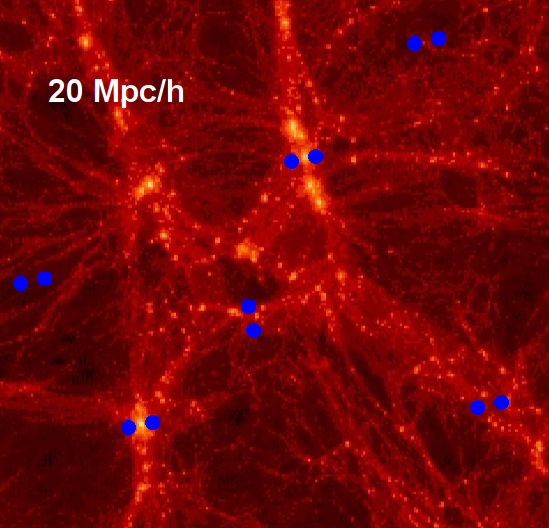
\includegraphics[trim = 0mm 0mm 0mm 0mm, clip, width=0.6\textwidth]
	{./figures/Pairs_in_Web.png}
\end{figure}
%.........................................................................
\end{block}
\end{frame}
%=========================================================================



%*****************************************************************************************************************
%			MOTIVACION
%*****************************************************************************************************************
\section{Construcción de las Simulaciones}
\label{sec:Simulations}
%=========================================================================
%FRAME 7
\begin{frame}
\begin{block}{Construcción de las Simulaciones: Resumen}\justifying

\begin{itemize}
\item Debido a las grandes escalas espaciales y temporales involucradas en la
evolución y dinámica del universo, se usan simulaciones numéricas como
laboratorios naturales.

\item La principal condición que deben satisfacer estos universos simulados 
es reproducir las observaciones.

\item Se asume como modelo de universo el modelo cosmológico estándar 
$\Lambda CDM$.
\end{itemize}

\end{block}
\end{frame}
%=========================================================================
%FRAME 8
\begin{frame}
\begin{block}{Construcción de las Simulaciones: Régimen Lineal}\justifying

A muy grandes escalas, se asume que el universo es homogéneo e isotrópico,
satisfaciendo las soluciones de Friedman para las ecuaciones de campo de 
Einstein.

%.........................................................................
%Friedman
\begin{figure}[htbp]
	\centering
	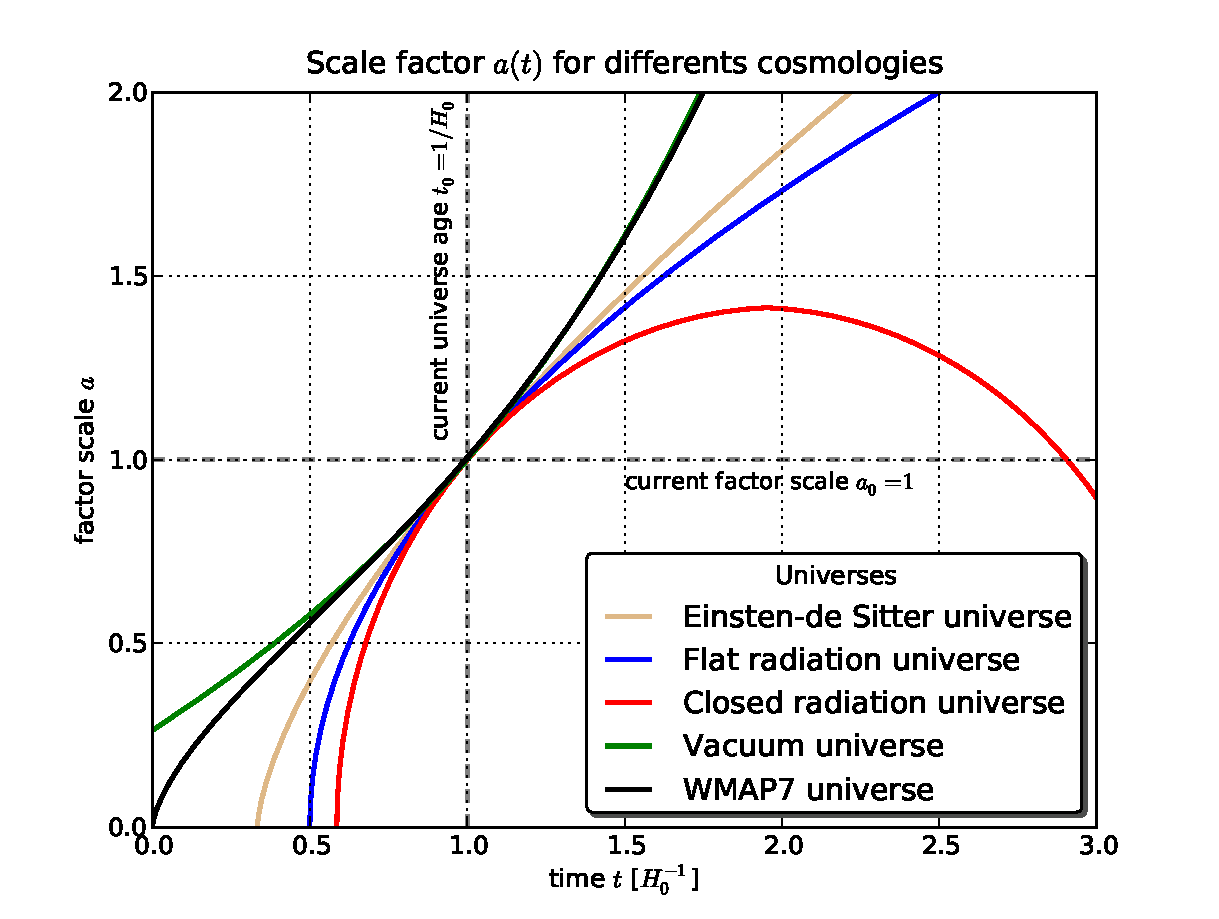
\includegraphics[trim = 0mm 0mm 0mm 0mm, clip, width=0.7\textwidth]
	{./figures/Friedmann_Solution.pdf}
\end{figure}
%.........................................................................

\end{block}
\end{frame}
%=========================================================================
%FRAME 9
\begin{frame}
\begin{block}{Construcción de las Simulaciones: Régimen Lineal}\justifying

\begin{itemize}
\item A partir de observaciones de supernovas distantes y galaxy redshift 
survey se ha establecido la consistencia del universo real con los modelos 
de Friedman (universo en expansión acelerada y uniforme). 


\item Lo anterior solo es válido en escalas grandes, siendo nosotros la 
principal prueba en contra de la condición de isotropía y homogeneidad.


\item Se hace evidente que es necesario introducir perturbaciones en la 
solución de fondo.
\end{itemize}

\end{block}
\end{frame}
%=========================================================================
%FRAME 10
\begin{frame}
\begin{block}{Construcción de las Simulaciones: Régimen Lineal}\justifying

\begin{itemize}
\item En estadios tempranos del universo, la distribución de materia y 
energía eran homogéneas, pero debido a las fluctuaciones cuánticas de vacío
de los campos presentes y el periodo de inflación cósmica, se producen 
pequeñas perturbaciones de densidad.
\item El tiempo en el cual las perturbaciones son pequeñas $\delta \rho \ll 
\bar \rho$ es denominado régimen lineal de formación de estructuras.
\item Este puede ser resuelto en una aproximación Newtoniana a partir de 
ecuaciones de fluidos.
\end{itemize}

\end{block}
\end{frame}
%=========================================================================
%FRAME 11
\begin{frame}
\begin{block}{Construcción de las Simulaciones: Régimen Lineal}\justifying

Los dos principales resultados del régimen lineal son:

\begin{itemize}
\item[\textbf{1.}] Acorde al modelo inflacionario, los modos normales del 
campo de densidad primigenio $\delta_{\bds k}$ se distribuyen normalmente 
siguiendo un espectro de potencia de Harrison-Zeldovich.

%.........................................................................
%Gaussian Distribution
\eq{eq:GaussianDistribution}
{ g_{\bds k}( r_{\bds k}, \phi_{\bds k}; t ) = 
\frac{2(r_{\bds k} dr_{\bds k})}{\sigma_k^2}\pr{ \frac{d\phi_{\bds k}}{2\pi} }
\exp\pr{ -\frac{r_{\bds k}^2}{\sigma_k^2} };\ \ \ \ \ \sigma_k^2 = 2\mu_k^2  }
%.........................................................................

\end{itemize}

\end{block}
\end{frame}
%=========================================================================
%FRAME 12
\begin{frame}
\begin{block}{Construcción de las Simulaciones: Régimen Lineal}\justifying

Distribución de Condiciones Iniciales

%.........................................................................
%Initial Density
\begin{figure}[htbp]
	\centering
	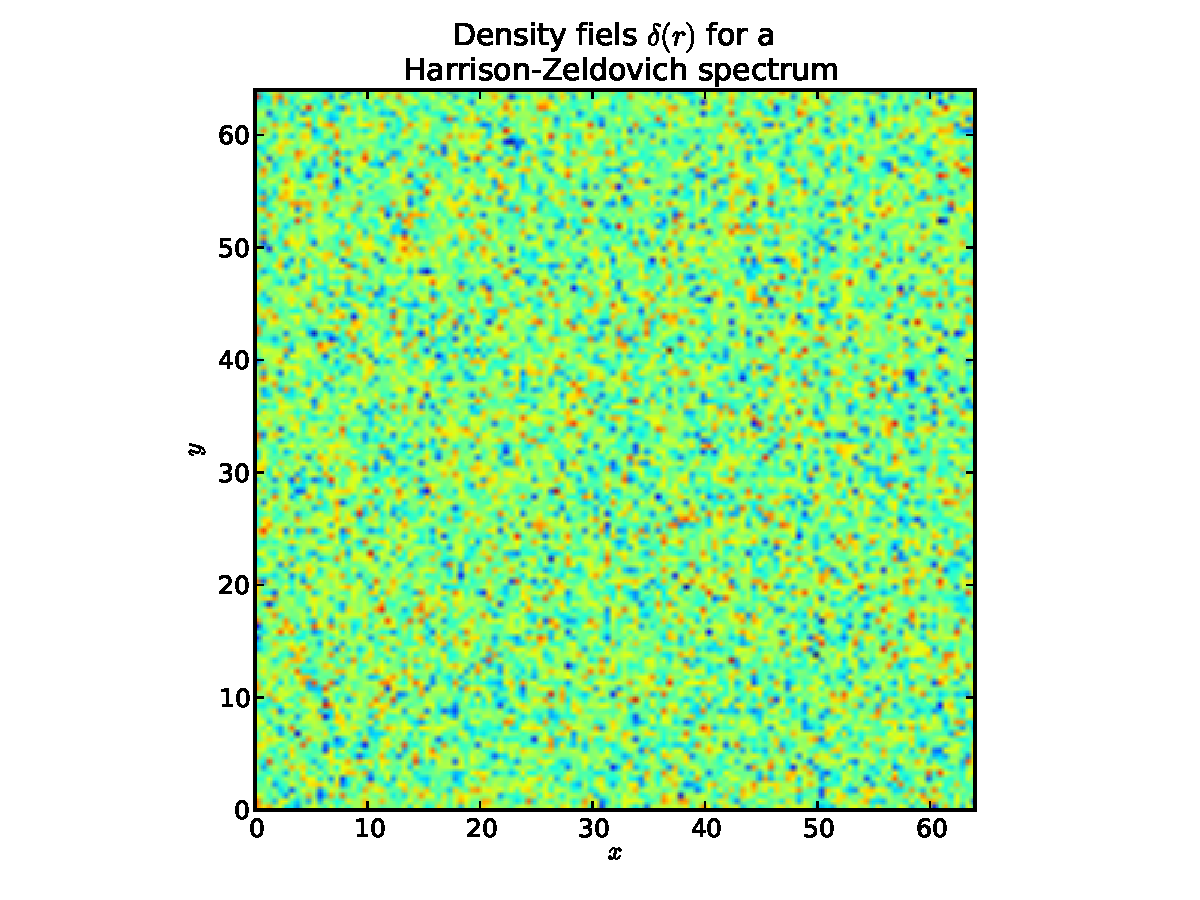
\includegraphics[trim = 0mm 0mm 0mm 0mm, clip, width=0.7\textwidth]
	{./figures/Initial_Density.pdf}
\end{figure}
%.........................................................................

\end{block}
\end{frame}
%=========================================================================
%FRAME 13
\begin{frame}
\begin{block}{Construcción de las Simulaciones: Régimen Lineal}\justifying

\begin{itemize}
\item[\textbf{2.}] El segundo resultado es la obtención de la función de 
transferencia, la cual permite conocer la evolución del universo en régimen
lineal

%.........................................................................
%Transfer
\begin{figure}[htbp]
	\centering
	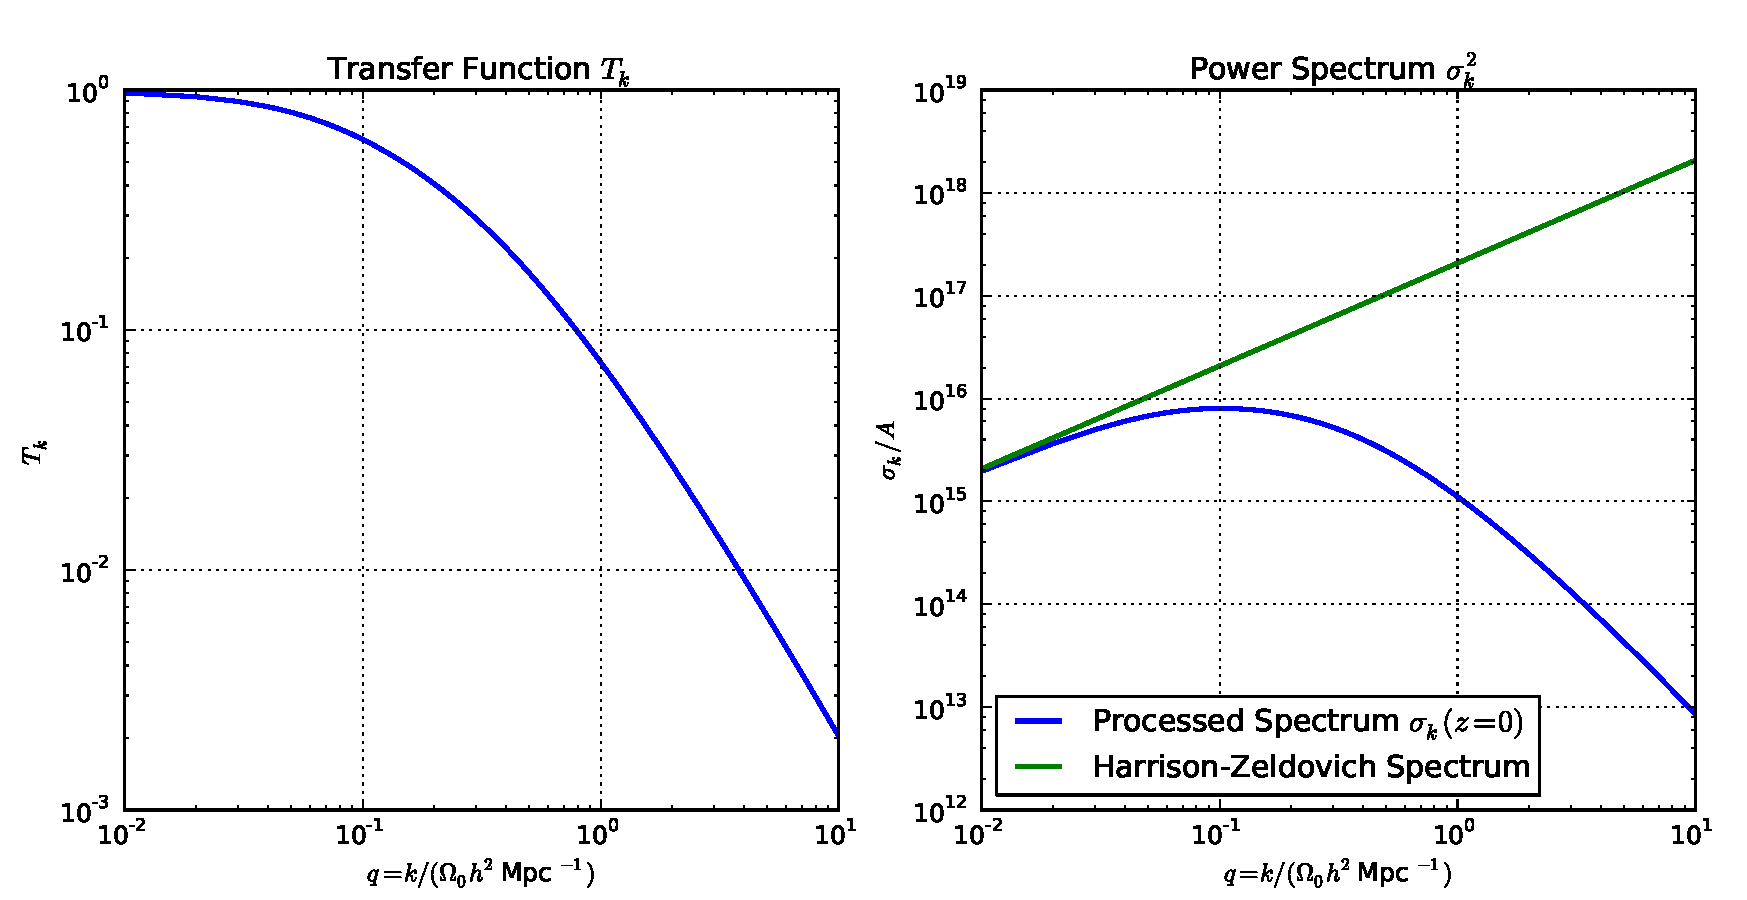
\includegraphics[trim = 0mm 0mm 0mm 0mm, clip, width=0.8\textwidth]
	{./figures/Transfer_Function.pdf}
\end{figure}
%.........................................................................

\end{itemize}

\end{block}
\end{frame}
%=========================================================================
%FRAME 14
\begin{frame}
\begin{block}{Construcción de las Simulaciones: Régimen No Lineal}\justifying

\begin{itemize}
\item A partir del colapso de Jeans, las perturbaciones crecen 
considerablemente respecto a la densidad media de fondo $\delta \rho \gg 
\bar \rho$.
\item Este periodo del universo es conocido como régimen no lineal.
\item Los procesos físicos involucrados ahora son altamente complejos, y un
desarrollo analítico análogo al régimen lineal no es posible, necesitado 
de simulaciones numéricas.
\end{itemize}

\end{block}
\end{frame}
%=========================================================================
%FRAME 15
\begin{frame}
\begin{block}{Construcción de las Simulaciones: Régimen No Lineal}\justifying

%.........................................................................
%Non linear evolution
\begin{figure}[htbp]
	\centering
	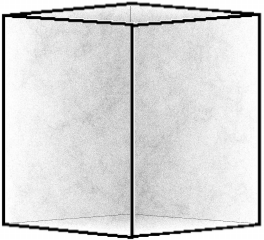
\includegraphics[trim = 0mm 0mm 0mm 0mm, clip, width=0.6\textwidth]
	{./figures/Nonlinear1.png}
\end{figure}
%.........................................................................

\end{block}
\end{frame}
%=========================================================================
%FRAME 16
\begin{frame}
\begin{block}{Construcción de las Simulaciones: Régimen No Lineal}\justifying

%.........................................................................
%Non linear evolution
\begin{figure}[htbp]
	\centering
	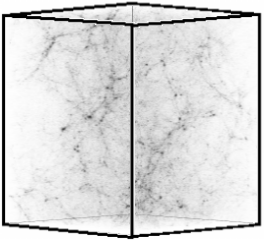
\includegraphics[trim = 0mm 0mm 0mm 0mm, clip, width=0.6\textwidth]
	{./figures/Nonlinear2.png}
\end{figure}
%.........................................................................

\end{block}
\end{frame}
%=========================================================================
%FRAME 17
\begin{frame}
\begin{block}{Construcción de las Simulaciones: Régimen No Lineal}\justifying

%.........................................................................
%Non linear evolution
\begin{figure}[htbp]
	\centering
	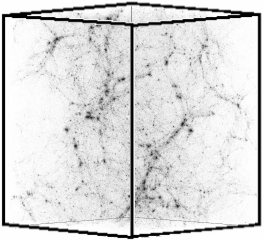
\includegraphics[trim = 0mm 0mm 0mm 0mm, clip, width=0.6\textwidth]
	{./figures/Nonlinear3.png}
\end{figure}
%.........................................................................

\end{block}
\end{frame}
%=========================================================================
%FRAME 18
\begin{frame}
\begin{block}{Construcción de las Simulaciones: Régimen No Lineal}\justifying

%.........................................................................
%Non linear evolution
\begin{figure}[htbp]
	\centering
	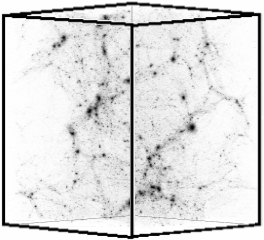
\includegraphics[trim = 0mm 0mm 0mm 0mm, clip, width=0.6\textwidth]
	{./figures/Nonlinear4.png}
\end{figure}
%.........................................................................

\end{block}
\end{frame}
%=========================================================================
%FRAME 19
\begin{frame}
\begin{block}{Construcción de las Simulaciones: Régimen No Lineal}\justifying

El régimen no lineal esta caracterizado por dos principales propiedades

\begin{itemize}
\item Una estructura jerárquica de formación de estructuras, donde estructuras
más pequeñas se forman primero y a partir de agrupación de estas se forman
las más grandes.
\item La aparición de la red cósmica, una estructura altamente inhomogénea
y anisotrópica en escalas pequeñas ($\sim$ Mpc), mientras es más homogénea
e isotrópica a grandes escalas. Es caracterizada por filamentos que se unen
en nodos de alta densidad, y permeada por regiones de alto vacío.
\end{itemize}

\end{block}
\end{frame}
%=========================================================================
%FRAME 20
\begin{frame}
\begin{block}{Construcción de las Simulaciones: Régimen No Lineal}\justifying
%.........................................................................
%Vweb
\begin{figure}[htbp]
	\centering
	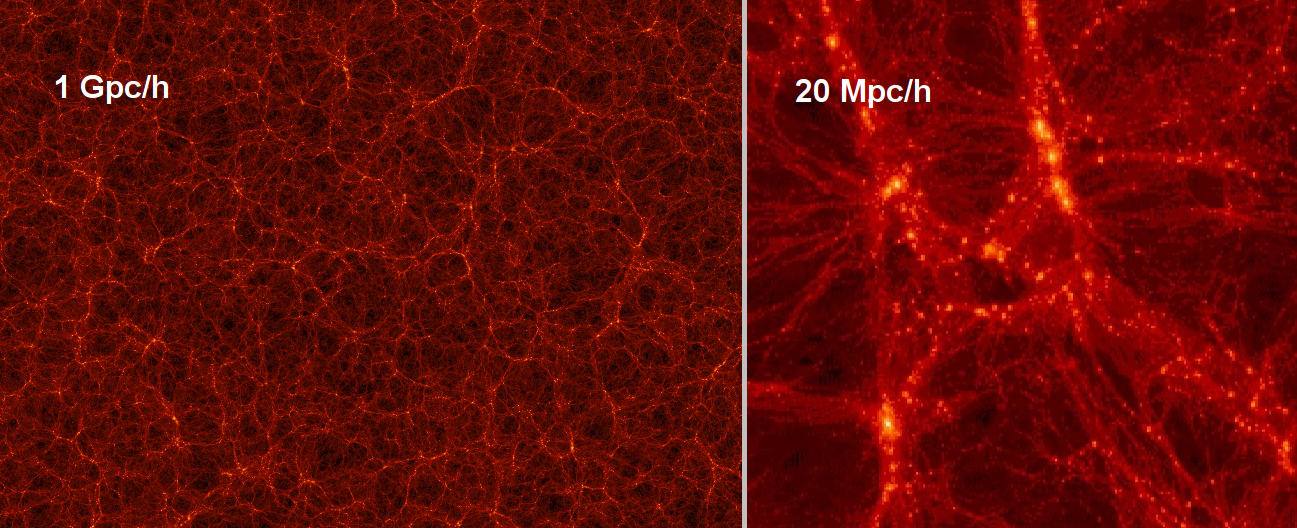
\includegraphics[trim = 0mm 0mm 0mm 0mm, clip, width=1.0\textwidth]
	{./figures/Web.png}
\end{figure}
%.........................................................................
\end{block}
\end{frame}
%=========================================================================
%FRAME 21
\begin{frame}
\begin{block}{Construcción de las Simulaciones: Régimen No Lineal}\justifying

La red cósmica ha sido también establecida a partir de redshift surveys
(SLOAN digital sky survey)

%.........................................................................
%SDSS
\begin{figure}[htbp]
	\centering
	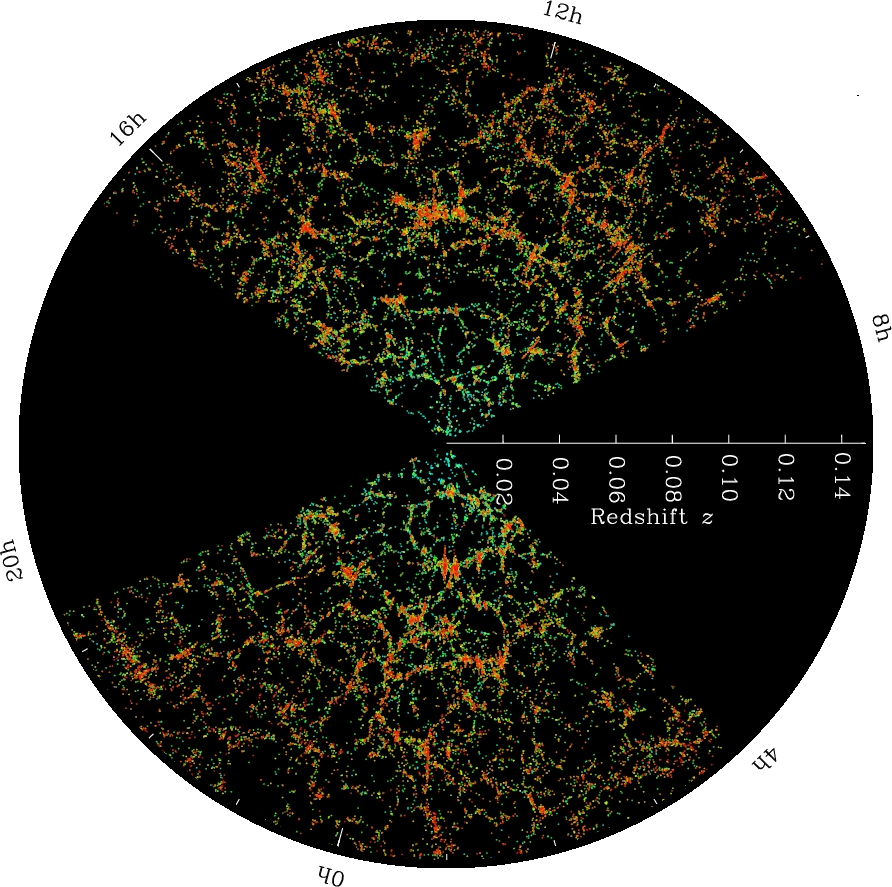
\includegraphics[trim = 0mm 0mm 0mm 0mm, clip, width=0.5\textwidth]
	{./figures/SDSS.png}
\end{figure}
%.........................................................................
\end{block}
\end{frame}
%=========================================================================
%FRAME 22
\begin{frame}
\begin{block}{Construcción de las Simulaciones: Tipos de Simulación}\justifying

Acorde a la esquema de construcción de las condiciones iniciales, las 
simulaciones se catalogan en dos tipos

\begin{itemize}
\item \textbf{Simulaciones No Restringidas:} son aquellas en las que las 
condiciones iniciales son construidas de forma aleatoria (fase aleatoria) 
siguiendo la distribución gaussiana establecida en el régimen lineal.
En este trabajo es usada la simulación Bolshoi.
\item \textbf{Simulaciones Restringidas:} son aquellas en las que las 
condiciones iniciales son construidas para reproducir el universo local
actual. Se usan tres simulaciones del proyecto CLUES.
\end{itemize}

\end{block}
\end{frame}
%=========================================================================
%FRAME 23
\begin{frame}
\begin{block}{Construcción de las Simulaciones: Tipos de Simulación}\justifying

\textbf{Simulación Bolshoi}

Esta es usada para aportar la estadística significativa debido a su tamaño
mayor respecto a las simulaciones restringidas ( $250 h^{-1}$ Mpc respecto a
$64 h^{-1}$ Mpc de las CLUES).

%.........................................................................
%Bolshoi
\begin{figure}[htbp]
	\centering
	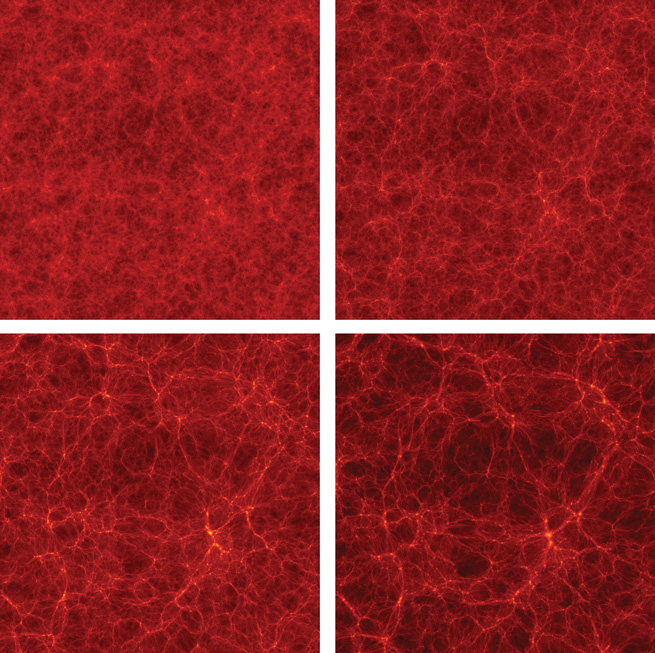
\includegraphics[trim = 0mm 0mm 0mm 0mm, clip, width=0.5\textwidth]
	{./figures/Bolshoi_Evolution.png}
\end{figure}
%.........................................................................

\end{block}
\end{frame}
%=========================================================================
%FRAME 24
\begin{frame}
\begin{block}{Construcción de las Simulaciones: Tipos de Simulación}\justifying

\textbf{Simulación CLUES}

Las tres simulaciones CLUES están construidas para reproducir el universo
local actual, en especial puede ser identificado el grupo local con 
aproximadamente la misma distribución de estructuras vecinas.

%.........................................................................
%CLUES
\begin{figure}[htbp]
	\centering
	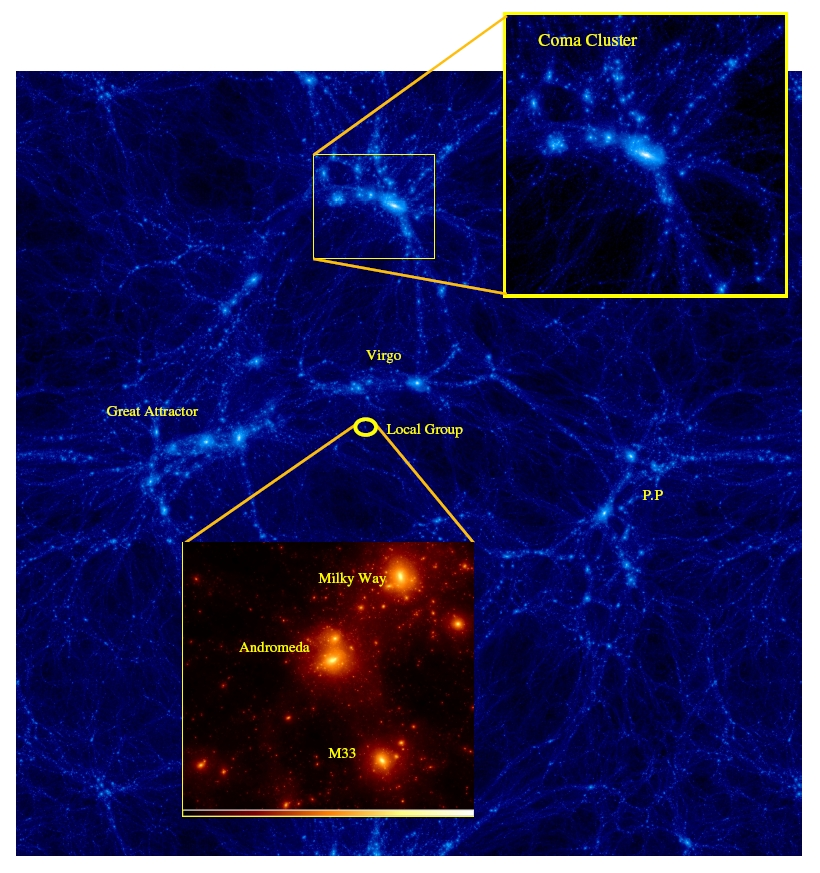
\includegraphics[trim = 0mm 0mm 0mm 0mm, clip, width=0.45\textwidth]
	{./figures/CLUES_Overview.png}
\end{figure}
%.........................................................................

\end{block}
\end{frame}
%=========================================================================
%FRAME 25
\begin{frame}
\begin{block}{Construcción de las Simulaciones: Cuantificación de la Red Cósmica}
\justifying

La cuantificación de la red cósmica se hace a partir del esquema V-web, este
hace uso del shear velocity tensor definido por:

%.........................................................................
\eq{eq:Vweb}
{ \Sigma_{ij} = -\frac{1}{2H_0}\pr{ \der{v_i}{r_j} + \der{v_j}{r_i} } }
%.........................................................................

Los autovalores de este tensor determinan la naturaleza de
colapso/expansión en las autodirecciones respectivas, esto permite construir
un esquema de clasificación.

\end{block}
\end{frame}
%=========================================================================
%FRAME 26
\begin{frame}
\begin{block}{Construcción de las Simulaciones: Tipos de Simulación}\justifying

%.........................................................................
%Scheme Clas
\begin{figure}[htbp]
	\centering
	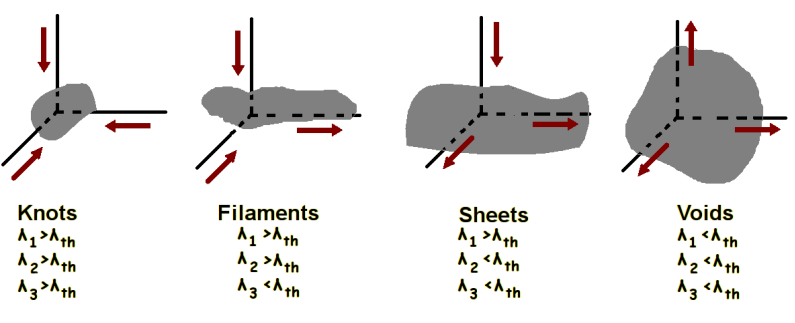
\includegraphics[trim = 0mm 0mm 0mm 0mm, clip, width=0.8\textwidth]
	{./figures/EnvironmentClassification.png}
\end{figure}
%.........................................................................

\end{block}
\end{frame}
%=========================================================================
%FRAME 27
\begin{frame}
\begin{block}{Construcción de las Simulaciones: Tipos de Simulación}\justifying

Acorde al valor umbral escogido $\lambda_{th}$ se obtienen diferentes 
impresiones visuales de las simulaciones, siendo $\lambda_{th} = 0.3$ la
que más se asemeja al campo de densidad.

%.........................................................................
%Scheme Clas
\begin{figure}[htbp]
	\centering
	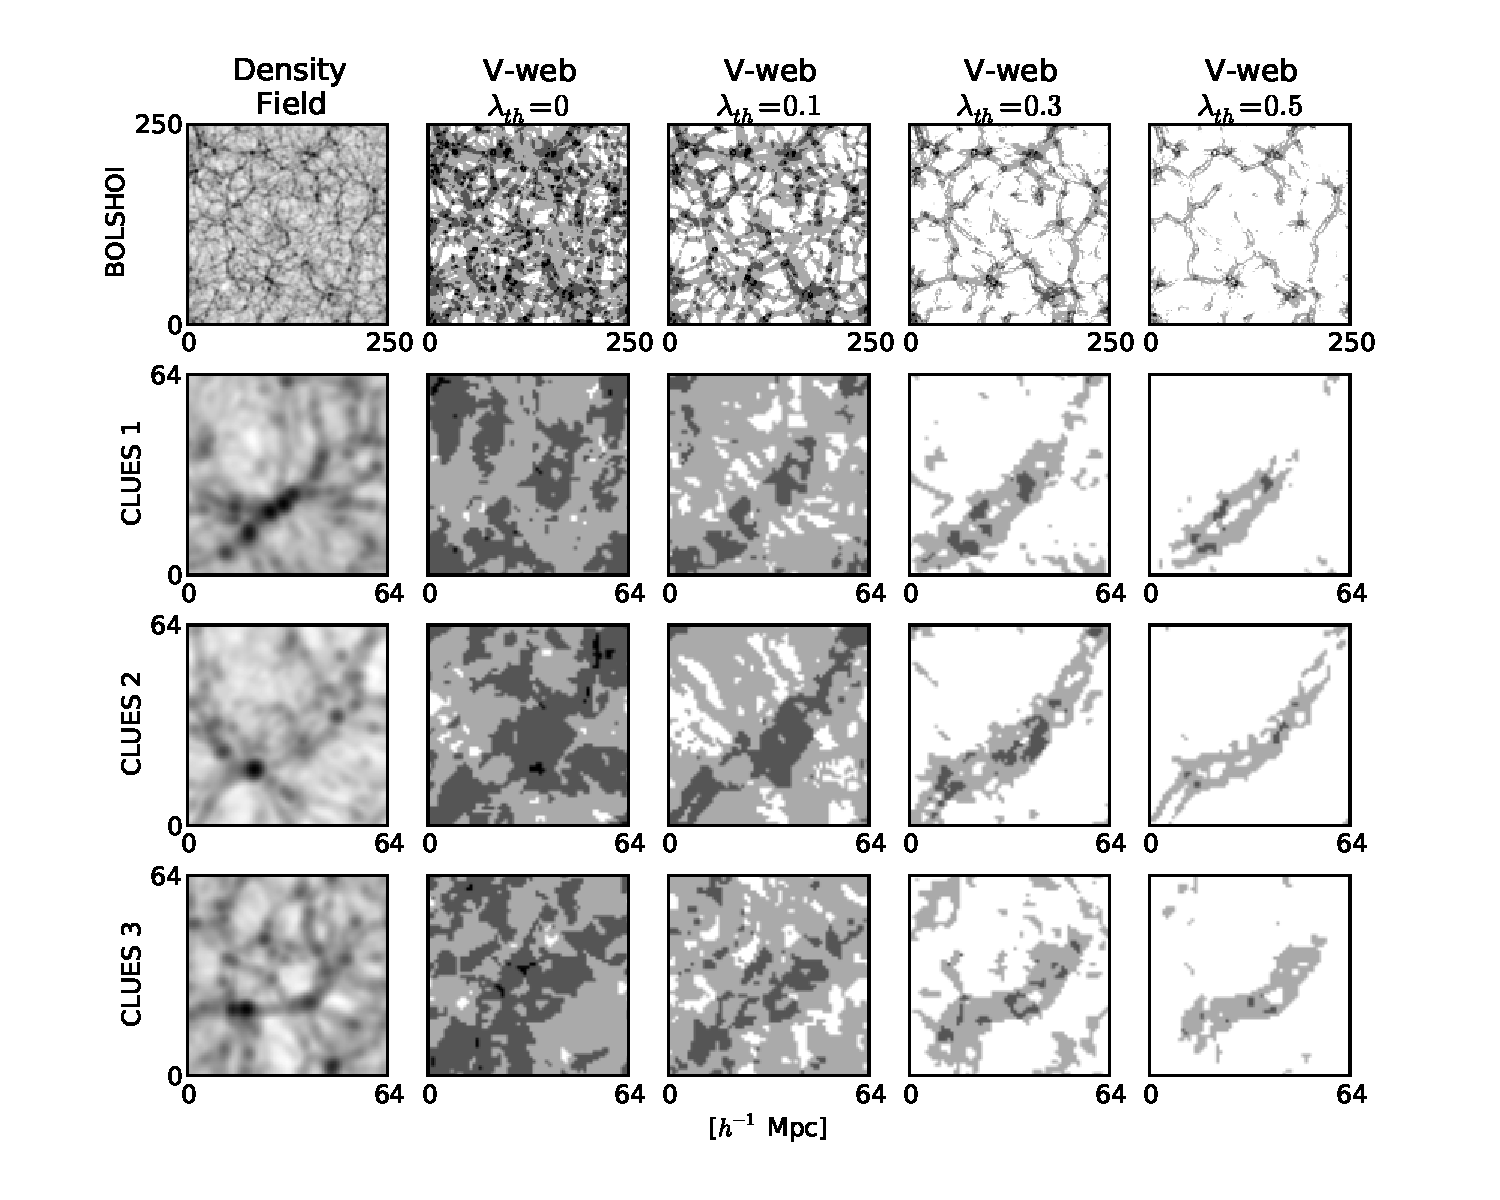
\includegraphics[trim = 0mm 10mm 0mm 10mm, clip, width=0.8\textwidth]
	{./figures/Vweb_Comparison.pdf}
\end{figure}
%.........................................................................

\end{block}
\end{frame}
%=========================================================================
%FRAME 28
\begin{frame}
\begin{block}{Construcción de las Simulaciones: Definición de Muestras}\justifying

Una vez caracterizado el entorno cosmológico de cada simulación, se procede
a definir las muestras a usar.

\begin{itemize}

\item \textbf{General Halos [\textit{GH}]:} Son todos los halos de materia 
oscura construidos a partir del esquema FOF (Friend of Friend).

\item \textbf{Halos Individuales [\textit{IH}]:} Son todos los halos de materia 
oscura en el rango de masa $5.0 \times 10^{11}\Msun - 5.0\times 10 ^{12}\Msun$.
Este rango favorece la formación de galaxias de disco.

\item \textbf{Pares [\textit{P}]:} esta es construida a partir de 
la muestra \textit{IH} y está compuesta por pares de halos que satisfacen el 
criterio de ser mutuamente el halo más cercano al otro.

\end{itemize}

\end{block}
\end{frame}
%=========================================================================
%FRAME 29
\begin{frame}
\begin{block}{Construcción de las Simulaciones: Definición de Muestras}\justifying

\begin{itemize}


\item \textbf{Pares Aislados [\textit{IP}]:} esta muestra se construye
a partir de los sistemas en la muestra de pares que además satisfacen las 
siguientes condiciones

%.........................................................................
%CLG conditions
	\begin{itemize}
	\item La distancia entre el centro de los halos debe ser menor a 
	$0.7 h^{-1}$ Mpc, consistente con la distancia entre la Vía Láctea
	y Andrómeda.
	\item La velocidad radial relativa entre ambos halos debe ser negativa.
	\item No debe haber ningún objeto más masivo que alguno de los dos halos
	a una distancia menor que $2.0 h^{-1}$ Mpc de ambos.
	\item No debe existir ningún objeto más masivo que $5.0 \times 10^{13}\Msun$
	a una distancia menor que $5h^{-1}$ Mpc respecto a ambos halos.
	\end{itemize}
%.........................................................................	
	
\item \textbf{Grupos Locales [\textit{LG}]:} esta muestra es 
definida en la simulaciones CLUES y corresponde a los pares de halos 
construidos a priori para la reproducción del grupo local. Por definición, 
solo existe un sistema \textit{LG} por cada una de las tres simulaciones 
CLUES.	
	
\end{itemize}

\end{block}
\end{frame}
%=========================================================================
%FRAME 30
\begin{frame}
\begin{block}{Construcción de las Simulaciones: Definición de Muestras}\justifying

\begin{itemize}

\item \textbf{Grupos Locales Construidos [\textit{CLG}]:} con el
objetivo de obtener una muestra de sistemas tipo \textit{LG} en 
simulaciones no restringidas, se propone un método de construcción basado
en el entorno cosmológico de la muestra \textit{LG} en las simulaciones 
CLUES. Para esto se calculan los 3 campos de autovalores del 
\textit{shear velocity tensor} en una malla con resolución de 
$1.0 h^{-1}$ Mpc/celda y un suavizado Gaussiano de una celda.

\end{itemize}

\end{block}
\end{frame}
%=========================================================================
%FRAME 31
\begin{frame}
\begin{block}{Construcción de las Simulaciones: Definición de Muestras}\justifying

%.........................................................................
%LG CLUES
\begin{figure}[htbp]
	\centering
	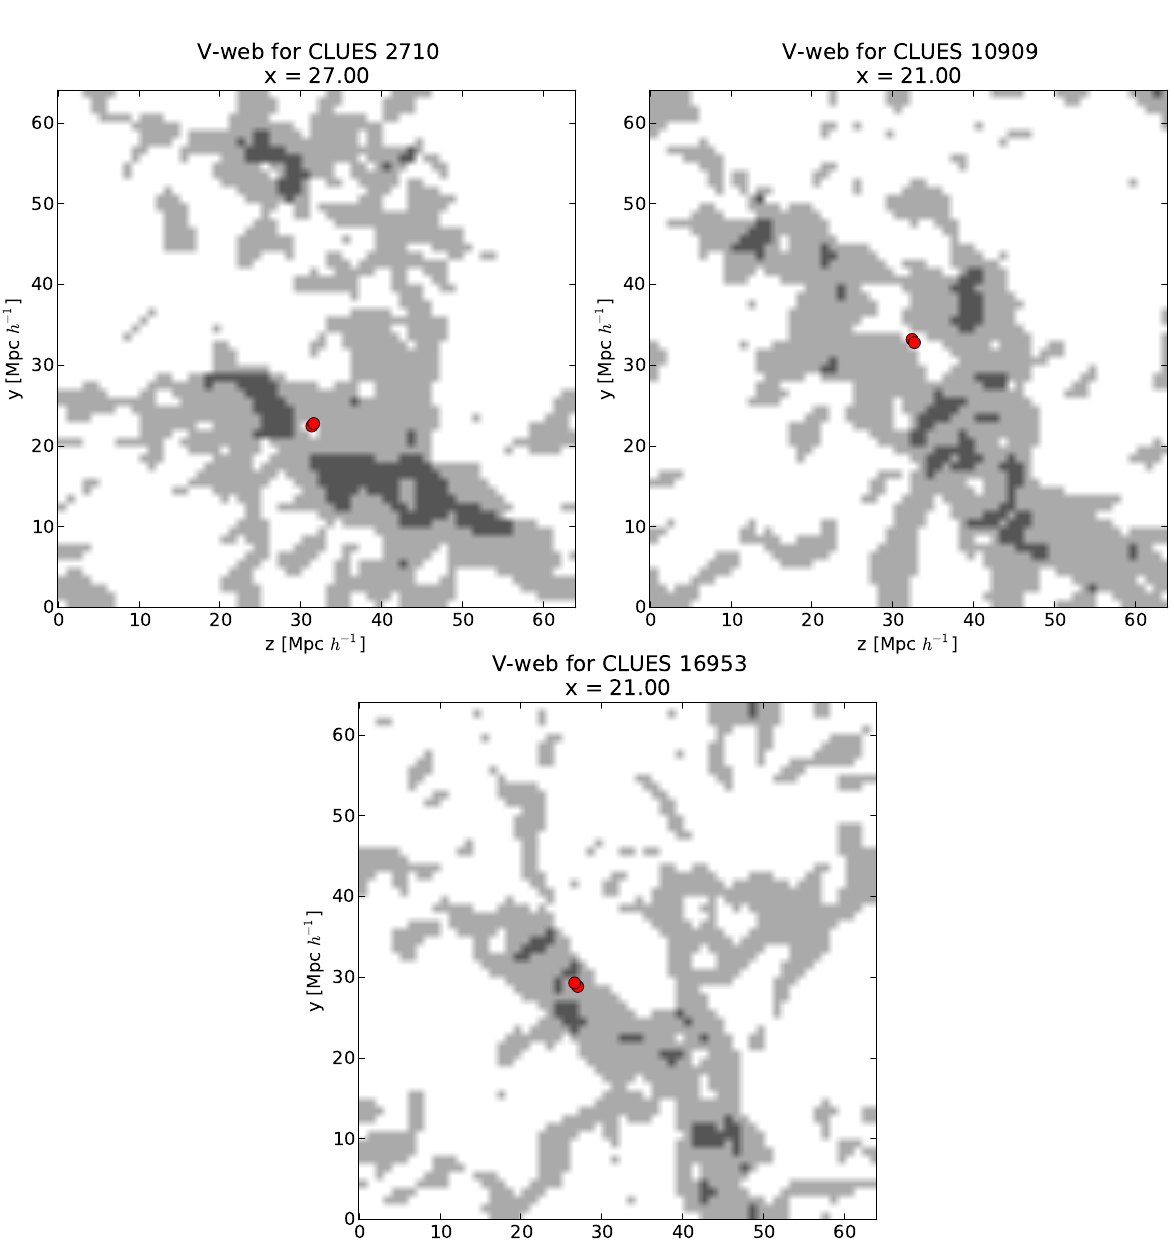
\includegraphics[trim = 0mm 10mm 0mm 10mm, clip, width=0.45\textwidth]
	{./figures/LG_Environment.png}
\end{figure}
%.........................................................................

\end{block}
\end{frame}
%=========================================================================
%FRAME 32
\begin{frame}
\begin{block}{Construcción de las Simulaciones: Definición de Muestras}\justifying

%.........................................................................
%LG CLUES
\begin{figure}[htbp]
	\centering
	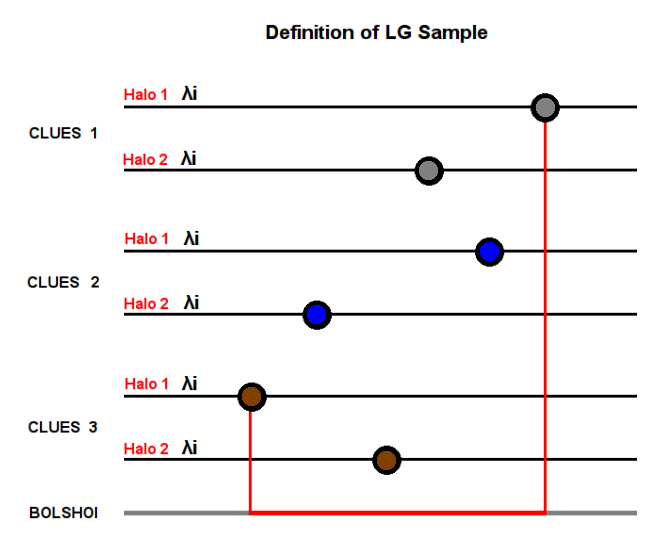
\includegraphics[trim = 0mm 0mm 0mm 0mm, clip, width=0.6\textwidth]
	{./figures/LG_definition.png}
\end{figure}
%.........................................................................

\end{block}
\end{frame}
%=========================================================================
%FRAME 33
\begin{frame}
\begin{block}{Construcción de las Simulaciones: Definición de Muestras}\justifying

%.........................................................................
%Table of samples numbers
\begin{table}[htbp]
\begin{small}
  \centering
  \begin{tabular}{| c | c | c | c | c |} \hline
	{\textbf{Muestra}}		& 
	{\textbf{CLUES 1}}		& 
	{\textbf{CLUES 2}} 		& 
	{\textbf{CLUES 3}}		& 
	{\textbf{Bolshoi}}		 \\ \hline
	\textit{GH} 	& 56632 & 57707 & 56799  & 432000 	\\
	\textit{IH}		& 1493 	& 1490 	& 1493	 & 88068 	\\
	\textit{P}		& 386 	& 380 	& 387	 & 23037 	\\
	\textit{IP}		& 20 	& 12 	& 18 	 & 1256 	\\
	\textit{LG}		& 1 	& 1 	& 1 	 & --		\\
	\textit{CLG}	& 1 	& 2 	& 3 	 & 30		\\ \hline
  \end{tabular}
  
  \caption{Tamaños de las muestras definidas para cada una de las 
  simulaciones. }  
  \label{tab:Samples}
\end{small}
\end{table}
%.........................................................................

\end{block}
\end{frame}
%=========================================================================


%*****************************************************************************************************************
%			GRACIAS!
%*****************************************************************************************************************
\begin{frame}
\begin{block}{}\justifying

\begin{huge}
\begin{center}
Muchas Gracias!
\end{center}
\end{huge}


\end{block}
\end{frame}
%=================================================================================================================


\end{document}